\documentclass[12pt,pra,aps]{revtex4}
\usepackage[dvipdfmx]{graphicx}
\usepackage[dvipdfmx]{color}
\usepackage[version=3]{mhchem}
\usepackage{float}
\usepackage{rotating}
\usepackage{array}
\usepackage{amsmath}
\usepackage{multirow}
\usepackage{setspace}
\usepackage{braket}
\usepackage{epstopdf}
\usepackage{moreverb}
\usepackage{wrapfig}

\usepackage{color}                            
                                              
\newcommand{\red}[1]{\textcolor{red}{#1}}     
\newcommand{\blue}[1]{\textcolor{blue}{#1}}

\newcommand{\boxz}[1]{\boxed{\phantom{\text{#1}}}}
\newcommand{\boxa}[1]{\boxed{\phantom{}}}

%%\renewcommand{\baselinestretch}{2.0}

\renewcommand{\thefigure}{S\arabic{figure}}
\renewcommand{\thetable}{S\arabic{table}}

\begin{document}
\title{分子軌道と分子の構造 \\(水素分子イオンとH\"uckel分子軌道法)}
\author{齋藤 雅明 \\ 量子化学研究室 \\ email: masa.saitow@chem.nagoya-u.ac.jp}

\maketitle

% Nakai & Ando, p. 68
\noindent
{\bf 問題1.} 1,3-ブタジエンとシクロブタジエンの共鳴安定化をH\"uckel法により考察する。
    
\noindent
{\bf 1.(a)} ブタジエンに対する永年方程式を解き、4つのエネルギー準位を求めよ。また、それぞれのエネルギー準位に対する占有状態も答えよ。

\noindent
{\bf 1.(b)} ブタジエンの$\pi$電子の全エネルギー及び共鳴エネルギー\footnote{非局在化エネルギーとも呼ばれる。}を求めよ。

\noindent
{\bf 1.(c)} シクロブタジエンに対する永年方程式を解き、4つのエネルギー準位を求めよ。また、それぞれのエネルギー準位に対する占有状態も答えよ。

\noindent
{\bf 1.(d)} シクロブタジエンの$\pi$電子の全エネルギー及び共鳴エネルギーを求めよ。

\noindent
{\bf 1.(e)} ブタジエン及シクロブタジエンの全結合次数を計算せよ。

\begin{wrapfigure}{r}[9pt]{0.2\textwidth}
  \centering
  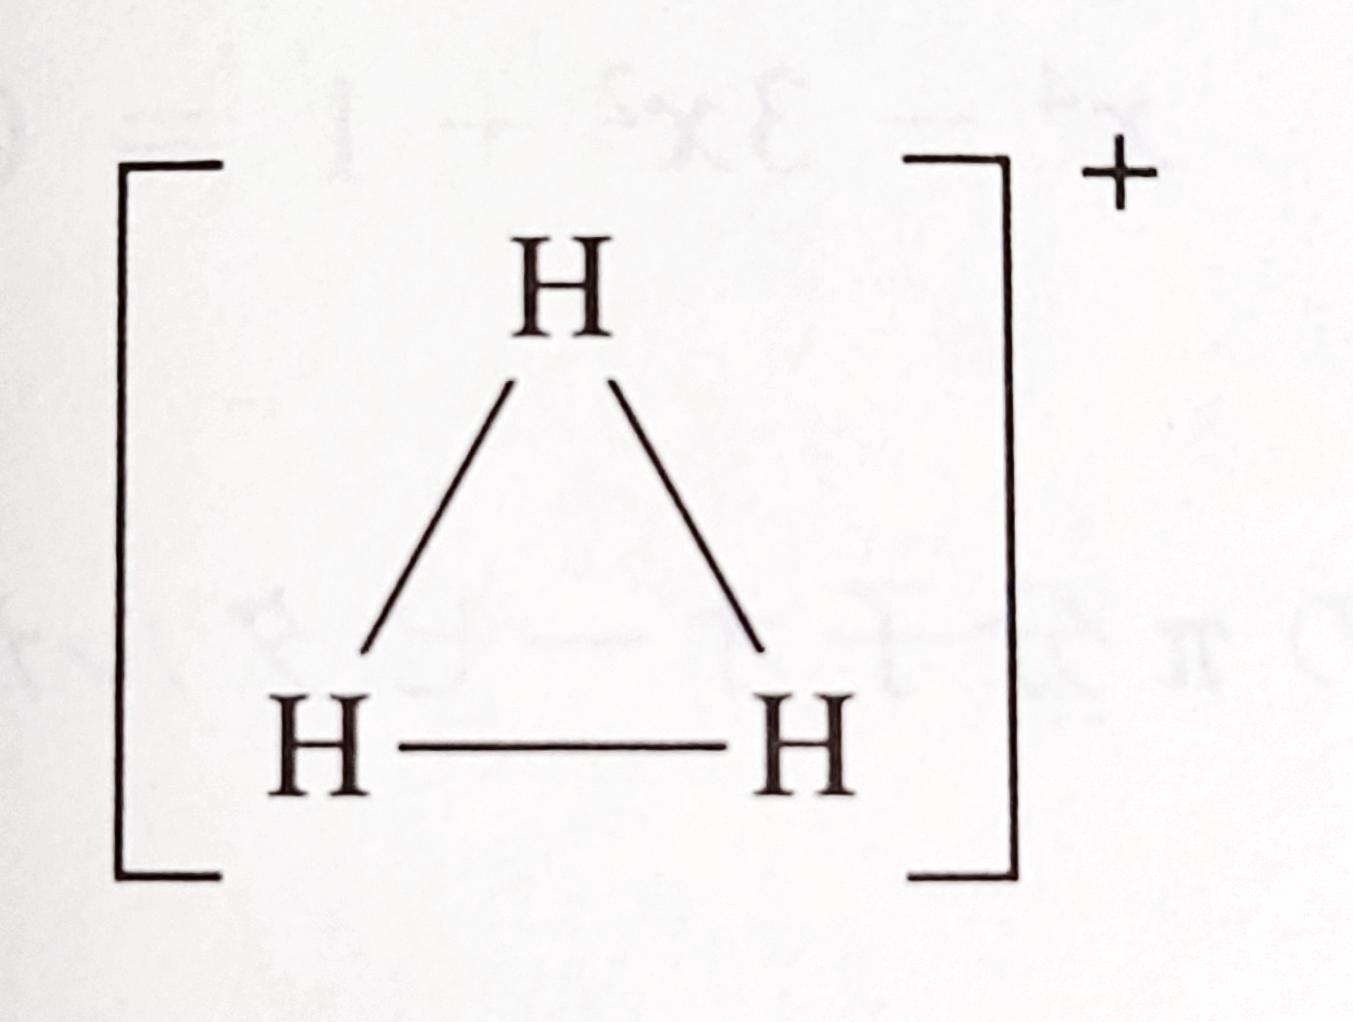
\includegraphics[width=3.0cm]{triangle.jpg}
  \caption{Triangular structure of \ce{H3+} molecule}
\end{wrapfigure}

% Nakai & Ando, p. 69
\noindent
{\bf 問題2.} ベンゼン\ce{C6H6}の$\pi$電子状態をH\"uckel法により考察する。

\noindent
{\bf 2.(a)} ベンゼンに対する永年方程式を解き、4つのエネルギー準位を求めよ。また、それぞれのエネルギー準位に対する占有状態も答えよ。

\noindent
{\bf 2.(b)} ベンゼンの6個の$\pi$電子は(a)で求めたエネルギー準位をどのように占有するか模式的に示せ。

\noindent
{\bf 2.(c)} ベンゼンの全エネルギー及び共鳴エネルギーを求めよ。

\noindent
{\bf 2.(d)} ベンゼンのイオン化エネルギー及び電子親和力を求めよ。

\noindent
{\bf 2.(e)} ベンゼンの共鳴エネルギーの実測値は209 kJ/mol${}^{-1}$である。この数値を再現するように、共鳴積分の値を決定せよ。また1,3-ブタジエンの共鳴エネルギーの実測値は43 kJ/mol${}^{-1}$である。このように決定された共鳴積分を用いた場合、エチレンの共鳴エネルギーはどのようになるか。

% McQuarrie p. 440, Prob. 10.37
\noindent
{\bf 問題3.} H\"uckel法によって、\ce{H3+}について直線構造と三角形構造のどちらが安定かを決定せよ。\ce{H3}と\ce{H3-}ではどうか。

\end{document}
